 \documentclass{beamer}

% MD: we can mess with this ...
%\usetheme{Berlin}
\usetheme{Goettingen}
% ... or use the IU style we've defined before:
%\usepackage{iucl}

\usepackage{multirow}

\usepackage{graphicx}
\usepackage{tikz-dependency}
\usepackage{natbib}
\usepackage{url}
\usepackage{gb4e}
\usepackage{tikz-qtree}

% workaround for weird \newblock problem
% http://www.isi.edu/~johnh/SOFTWARE/uclathes.html
\def\newblock{\hskip .11em plus .33em minus .07em}
%%%CLingDing abstract:
% We will be presenting work in progress for improving methods to semantically analyze interactive learner sentences.  In past experiments, we evaluated the semantic appropriateness of picture description task (PDT) responses from non-native speakers (NNSs) of English by using a rule-based system that compares these responses to those from native speakers (NSs). We found many problems in maintaining a thorough Gold Standard (GS) and thus in establishing the quality of NNS responses.

% Here we address these challenges by turning to more general approaches, involving more abstract representations of the data (e.g., dependency fragments), as well as gradability in the NNS responses, as opposed to a strict good/bad distinction.  After presenting experiments with a range of parameters, we will present work clustering the PDT items, based both on the input (NNS responses) and output (system performance).  In this way, we hope to find the best system settings for new PDT items and to get a better handle on the variability within learner language.

\title{Semantic Analysis of Image-Based \\ Learner Sentences}
\author[Levi King]{Levi King \\ Dissertation Proposal}
\date{Department of Linguistics, Indiana University \\ August 29, 2016}

\setbeamerfont{page number in head/foot}{size=\footnotesize}
\setbeamertemplate{footline}[frame number]

\begin{document}

\maketitle

\section{Motivation}
\begin{frame}
\frametitle{Motivation}

\textbf{Issue:}
\begin{itemize}
\item Intelligent Computer-Assisted Language Learning (ICALL) / Intelligent Language Tutor (ILT) systems tend to focus on grammatical errors \& feedback \citep{heift:schulze:07, meurers:12}. %\citep{meurers:12} 
 
\item Second Language Acquisition (SLA) research has established:
  \begin{itemize}
  \item Explicit grammar instruction \& feedback are often ineffective \citep{Ellis:2006:CurrentIssues}.
  \end{itemize} 
\end{itemize}

%\medskip

\textbf{Goals:} 
\begin{itemize}
\item Big Picture: Steer ICALL/ILT toward a focus on communication, with learners producing \textit{more} target language rather than perfectly formed target language.
\begin{itemize}
\item Requires better methods to provide semantic analysis of contextual learner sentences.
\end{itemize}
\item Current: Explore the viability of such analysis using existing tools and resources.
\end{itemize}

\end{frame}

%
%\begin{frame}
%\frametitle{Organization}
%
%\end{frame}

\begin{frame}
\frametitle{Motivation}
\framesubtitle{Previous Work}

\begin{itemize}
\item \textit{Herr Komissar}: ILT/detective game for German learners;
content analysis \& sentence generation \citep{desmedt:95}, but
uses many custom tools. 
\item \citet{petersen:10}: ILT, provides feedback on questions in English,
extracting meanings from an existing parser.
\item Content assessment: (e.g., ETS's c-rater system \citep{leacock:chodorow:03}); mostly focused on essay \& short answer scoring. 
  \begin{itemize}
  \item Some focus on semantic analysis under restricted conditions,
    e.g., \citep{Meurers.Ziai.ea-11}.
  \end{itemize}
\item \citet{somasundaran:chodorow:14}, \citet{somasundaran:ea:15}:
  score picture-based sentences \& narrations
  \begin{itemize}
  \item for relevance: calculate overlap of response contents with
    picture contents
  \item for picture contents: expert annotators listed all items in the
    picture \& wrote 5 sentences each
  \end{itemize}
\end{itemize}

\end{frame}

\begin{frame}
\frametitle{Motivation}
\framesubtitle{Reasoning about learner meaning}

%... maybe/maybe not have such a transition slide ...

Focusing on semantic analysis (feedback, scoring, etc.) means that one
should have a sense of:
\begin{itemize}
\item Semantic correctness / relevance of learner sentences
  \begin{itemize}
  \item ... vs. appropriateness / nativeness
  \end{itemize}
%\item Nativelikeness
\item Semantic variability in learner data
\end{itemize}

Still teasing these apart; forming annotation scheme

\bigskip

%One needs to account for 

Note that this is semantic analysis given a gold standard (GS) of
native sentences
\begin{itemize}
\item Image description often uses semantic primitives
  \citep{ortiz:wolff:lapata:15}
\item For learner data, we want to ensure that we can account not just
  for correct semantics (\emph{what}), but natural expressions of it
  (\emph{how})
  \begin{itemize}
  \item i.e., we need access to specific linguistic forms (GS)
  \end{itemize}
\end{itemize}

\end{frame}

\section{Background}

\begin{frame}
\frametitle{Background}
\framesubtitle{General approach}
I approximate the goal of an ICALL application that evaluates semantic accuracy and appropriateness by:
\begin{enumerate}
\item collecting data from a task which elicits contextual language use, namely a picture
description task (PDT),
\item parsing it with an off-the-shelf parser,
\item comparing NNS response dependencies with GS set of NS dependencies to get similarity score,
\item ranking NNS responses by score,
\item discriminating between acceptable and unacceptable responses based on rankings (\textit{work in progress})
\end{enumerate}

\medskip

\end{frame}

%\subsection{Data}
\begin{frame}
\frametitle{Background}
\framesubtitle{Data}
\footnotesize
\begin{figure}[width=0.8\columnwidth]
\begin{center}
\begin{tabular}{|c|}
\hline
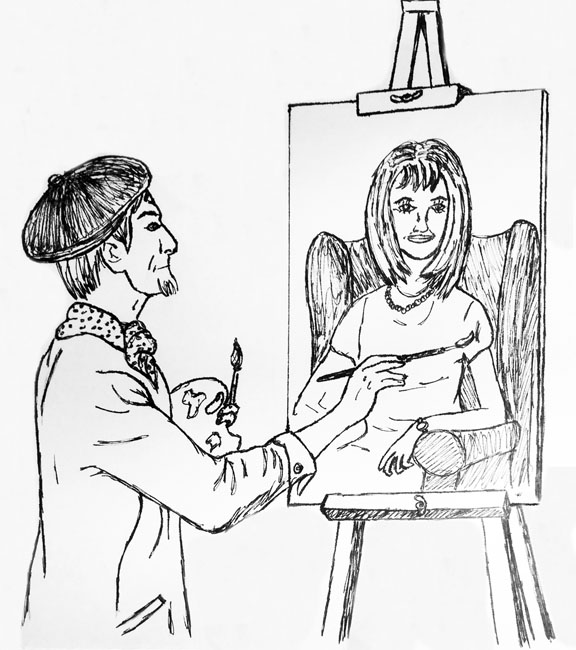
\includegraphics[width=0.4\columnwidth]{../figures/exampleprompt.jpg}\\
\hline
\textbf{Response (L1)}\\
\hline
He is droning his wife pitcher. (Arabic)\\
\hline
The artist is drawing a pretty women. (Chinese) \\
\hline
The artist is painting a portrait of a lady. (English) \\
\hline
The painter is painting a woman's paint. (Spanish)\\
\hline
\end{tabular}
\end{center}
\end{figure}
\begin{itemize}
\item 10 items, mostly transitives
\item 14 NSs, 39 NNSs
\end{itemize}
\end{frame}


\section{Research questions}

\begin{frame}
\frametitle{Research questions}
\framesubtitle{Overview}
\begin{enumerate}
{\item Are NSs \& NNSs similar enough for auto analysis?}
{\item How to represent responses internally?}
{\item Can existing tools \& resources be used effectively? Which ones?}
{\item Effectiveness of bag-of-words vs. bag-of-dependencies?}
{\item Can semantic tools improve performance?}
{\item Annotation scheme? System vs. human agreement?}
\end{enumerate}
\end{frame}

\begin{frame}
\frametitle{Research questions}
%Given both the practical need to develop a GS and the theoretical issues surrounding nativeness and ultimate attainment, the first research question is:
\begin{enumerate}
\uncover<1->{\item Are the responses of intermediate and advanced L2 English learners sufficiently similar to those of NSs to allow automatic evaluation based on a collection of NS responses? In other words, do learners demonstrate significant overlap with native-like usage in a PDT setting?}
%\end{enumerate}
%The images of the communication task serve as a rough simulation of real world scenes; given the lack (and desirability) of learner tools that analyze language content in visual contexts, the second research question is:
%\begin{enumerate}\setcounter{enumi}{1}
\medskip
\uncover<2->{\item In the constrained communicative environment of a PDT, what are appropriate response and GS representations for the purpose of providing meaning-oriented feedback or evaluation? In other words, which linguistic components are crucial and which are superfluous?}
\end{enumerate}
%As mentioned above, one goal of this project is to show that content-based evaluation of learner sentences is possible without the expense of developing major new tools or language resources; in this vein, the third research question is: 
\end{frame}

\begin{frame}
\frametitle{Research questions}
\begin{enumerate}\setcounter{enumi}{2}
\uncover<1->{\item What kinds of existing NLP tools and language resources can be integrated to form a content analysis system for open response language learning tasks?}
%\end{enumerate}
%As discussed later, this work attempts to take statistical methods traditionally used to analyze the frequencies of individual words in sentences and apply those methods to the frequencies of syntactic dependencies in sentences, as one means of deriving semantic information from syntactic tools. Thus, the fourth research question is:
%\begin{enumerate}\setcounter{enumi}{3}
\bigskip
\uncover<2->{\item How do ``bag-of-words'' and ``bag-of-dependencies'' approaches compare in terms of performance? Is a bag-of-words approach alone adequate for this task?}
\end{enumerate}
\end{frame}

\begin{frame}
\frametitle{Research questions}
%Given that the system has thus far relied primarily on a parser, lemmatizer and spelling correction module, without the inclusion of semantic tools, the fifth research question is: %and given NLP trends that focus on surface forms over deeper processing...
\begin{enumerate}\setcounter{enumi}{4}
\uncover<1->{\item Can the accuracy of the system be improved by the inclusion of semantic information from tools like semantic role labelers or WordNet?}
%\end{enumerate}
%%Are increases in performance valuable enough to offset the computational costs? In other words, how deep should the processing be in order to achieve our goal of providing a meaning-based ICALL component that is lightweight and practical?} %%%**How deep should the processing be?
%To evaluate the system, it will be necessary to have humans annotate the NNS responses, then compare this annotation to system output. In light of the specific nature of the PDT and the goal of analyzing semantic appropriateness, the sixth research question is:

%\begin{enumerate}\setcounter{enumi}{5}
\bigskip
\uncover<2->{\item What is the annotation scheme for this task and can the system perform within the range of inter-annotator reliability? Relatedly, what does it mean for a response to be \textit{appropriate} and how can this be captured with annotation?}
\end{enumerate}
\end{frame}

\section{Past work}

%\begin{frame}
%\frametitle{Past work}
%%\framesubtitle{Approach}
%%\begin{enumerate}
%%\item Preprocess to normalize responses: Spelling correction module \texttt{+} trigram language model; lemmatizer
%%\item Parse sentence with dependency parser 
%%\item Using custom rules, extract a semantic triple (S,V,O) from this parse
%%\item Compare to gold standard semantic forms
%%\end{enumerate}
%\begin{figure}
%\begin{center}
%    \begin{dependency}[arc edge,text only label,label style={above}]
%    \begin{deptext}[column sep=.5em]
%      \textit{vroot} \& The \&[1em] \textbf{boy} \&[1em] \textbf{played} \& with \& a \&[1em] \textbf{ball} \\
%    \end{deptext}
%    \depedge[label style={font=\bfseries,thick}]{4}{3}{nsubj}
%    \depedge[arc angle=90,label style={font=\bfseries,thick}]{1}{4}{root}
%    \depedge[label style={font=\bfseries,thick}]{4}{7}{prep\_with}
%    \depedge[arc angle=35]{7}{6}{det}
%    \depedge{3}{2}{det}
%  \end{dependency}
%\end{center}
%\label{fig:prep-dependency}
%\end{figure}
%\end{frame}

\begin{frame}
\frametitle{Past work}
\framesubtitle{Results}
\citet{king:dickinson:13} (no spelling correction):

\begin{itemize}
\item matched NNS S-V-O with NS S-V-O set (GS)
\item 92-93\% extraction accuracy (extracted correct S-V-O)
\item Among correctly extracted triples, we achieved 50.8\% coverage (153/301), 60.6\% accuracy (218/360)
\end{itemize}
\medskip
\citet{king:dickinson:14} (with spelling correction):
\begin{itemize}
\item Decreased errors by 13.7\% (*with potential for a decrease of 25.9\%)
\begin{itemize}
\item *Spelling correction is influenced by the GS, which is very limited here
\end{itemize}
\item Boosted coverage by 13.4\% (again, influenced by limited GS)
\end{itemize}
\end{frame}

\begin{frame}
\frametitle{Past work}
%\framesubtitle{Lingering issues}
\framesubtitle{Limitations}

There are several limitations to this past approach:
\medskip
\begin{itemize}
\item Incomplete data:
  \begin{itemize}
  \item The GS will always be missing innovations of learners
  \end{itemize}
  \smallskip
\item Incomplete rules
  \begin{itemize}
  \item Extraction rules do not generalize beyond transitives
  \end{itemize}
  \smallskip
\item Simplistic notion of non-native speaker data:
  \begin{itemize}
  \item Responses are not always simply right or wrong, but perhaps more
    or less relevant, nativelike, ...
  \end{itemize}
\end{itemize}

\medskip

\textbf{Dissertation work:} Addressing these limitations!

\end{frame}

\section{Dissertation work}

\begin{frame}
\frametitle{Dissertation work}
\framesubtitle{Remaining tasks}
\begin{itemize}
\small
\item Data collection: 25 items; more forms, participants
\item Annotation: scheme; guidelines; implementation \footnote{``[ ]'': Relevant research questions}[6]
\begin{itemize}
\item \footnotesize{inaccurate \textless \ accurate, not native-like \textless \ accurate + native-like}
\end{itemize}
\item Revise system to match new annotation scheme [2,6]
\item Run system on new data [1,6]
\item Integrate semantic role labeler \& WordNet; get results [3,4,5]
\item Clustering \& automatic parameter selection; new results [1,6]
\item Feedback module: provide user with most-similar NS response, most common NS response [2]
\end{itemize}
\end{frame}

\subsection{Representation}
\begin{frame}
\frametitle{Dissertation work}
\framesubtitle{Response representation}

%\vspace{-1.5em}

\textbf{Approach:} Generalize representations to overcome incomplete
GS by using dependencies

%Using dependencies per se is more robust than triples:
\begin{itemize}
\item Simpler than triples: no extraction rules or errors
\item Can distribute matching over smaller, overlapping pieces of info, not \textit{single, highly specific} piece of info (SVO)
\end{itemize}

\smallskip

Currently: List out all dependencies in response
\begin{itemize}
\item Full form (label\#dependent\#head): \texttt{nsubj\#boy\#play}
\item Plus partial abstractions: \texttt{nsubj\#X\#play}, etc.
%\texttt{(null)\#boy\#kick}, etc.} 
%  \begin{itemize}
%  \item We try each form separately, but may ultimately make use of
%    some weighted combination of these variations.
%  \end{itemize}
\begin{figure}
\begin{center}
    \begin{dependency}[arc edge,text only label,label style={above}]
    \begin{deptext}[column sep=.5em]
      \textit{vroot} \& The \&[1em] \textbf{boy} \&[1em] \textbf{played} \& with \& a \&[1em] \textbf{ball} \\
    \end{deptext}
    \depedge[label style={font=\bfseries,thick}]{4}{3}{nsubj}
    \depedge[arc angle=90,label style={font=\bfseries,thick}]{1}{4}{root}
    \depedge[label style={font=\bfseries,thick}]{4}{7}{prep\_with}
    \depedge[arc angle=35]{7}{6}{det}
    \depedge{3}{2}{det}
  \end{dependency}
\end{center}
\label{fig:prep-dependency}
\end{figure}
\end{itemize}
%
%\medskip
%Future representations might include:
%\begin{itemize}
%\item{lexical info (WordNet relations)}
%\item{SRL output (theta roles / verb argument indices)}
%\end{itemize}

\end{frame}

\subsection{Comparison}
\begin{frame}
\frametitle{Dissertation work}
\framesubtitle{Response and GS comparison}

\textbf{Approach:} Loosen the exact matching requirements \& use
frequency of terms to determine importance
\begin{itemize}
\item i.e., deduce relevancy from consistency among NSs
\end{itemize}

\medskip

Four ($2 \times 2$) comparison approaches:

\begin{itemize}
\item Term (i.e., lemmatized dependency or word) scores:
\begin{enumerate}
\item frequency; \textit{vs} 
\item tf-idf \footnote{term frequency-inverse document frequency; method for scoring importance of terms in a document by comparing frequencies in document to those in a general sample of the language}
\end{enumerate}
\item Response score:
\begin{enumerate}
\item assign NNS terms their scores in GS, then average; \textit{vs}
\item compare NNS \& GS term score vectors for cosine distance
\end{enumerate}
\end{itemize}
\end{frame}



\begin{frame}
\frametitle{Dissertation work}
\framesubtitle{Experiments}

Rather than \textit{match} / \textit{non-match} determination, current approaches give response scores ranging from 0--1.
\bigskip

Parameters:
\smallskip

\begin{enumerate}
\item term form (label/dep/head): ldh; \textit{x}dh; l\textit{x}h; ld\textit{x}
\begin{itemize}
\item \textit{OR} individual words (lemmatized)
\end{itemize}
\smallskip
%\item tf-idf reference corpus (TA \& TC only): Brown; WSJ
\item tf-idf reference corpus: Brown; WSJ
\medskip

\item NNS source: Original (NNSO); Version from spelling correction \texttt{+} LM (NNSLM)
\begin{itemize}
\item{Also planning joint analysis: both sources are considered and the one with the better score is selected.}
\end{itemize}
\end{enumerate}
\end{frame}

\begin{frame}
\frametitle{Dissertation work}
%\vspace{-.2em}
\framesubtitle{Ranking sentences}
\footnotesize{Each set of parameters produces a scored, ranked list of responses.}
\begin{center}
\scriptsize
\begin{table}
\begin{tabular}{|r|c|l|r|r|}
 \hline
 \textit{R} & \textit{S} & Sentence & \textit{E} & \textit{V}\\
 \hline
 \hline
\multirow{2}{*}{1} & 1.000 & she is hurting. & 1 & 1.5 \\
& 1.000 & man mull bird & 1 & 1.5 \\
\hline
3 & 0.996 & the man is hurting duck. & 1 & 3.0 \\
4 & 0.990 & he is hurting the bird. & 1 & 3.0 \\
\hline
11 & 0.865 & the man is trying to hurt a bird & 1 & 11.0 \\
12 & 0.856 & a man hunted a bird. & 0 & 0.0 \\
\hline
17 & 0.775 & the bird not shot dead.  & 1 & 17.0 \\
18 & 0.706 & he shot at the bird & 0 & 0.0 \\
19 & 0.669 & a bird is shot by a un & 1 & 19.0 \\
20 & 0.646 & the old man shooting the birds & 0 & 0.0 \\
\hline
37 & 0.086 & the old man shot a bird. & 0 & 0.0 \\
38 & 0.084 & a old man shot a bird. & 0 & 0.0 \\
39 & 0.058 & a man shot a bird & 0 & 0.0 \\
  \hline
  \hline
  \multicolumn{3}{|c|}{Total Raw Score (not normalized)} & 17 & 169 \\
  \hline
  \multicolumn{3}{|c|}{Average Precision} & \multicolumn{2}{c|}{0.75084} \\
 \hline
\end{tabular}
\end{table}
\end{center}
\footnotesize{\textit{R}: rank; \textit{S}: sentence score; \textit{E}: error; \textit{V}: rank value.
Item 10, best system setting (TC\_B\_NNSLM\_ldh) based on average precision scores.}

\end{frame}

\subsection{Data collection}
\begin{frame}
\frametitle{Dissertation work}
\framesubtitle{Data collection}
\begin{itemize}
\item 25 items; various forms, syntax
\item NSs provide 2 responses per item
\end{itemize}
\begin{figure}[width=0.9\columnwidth]
\begin{center}
%\begin{table}
\begin{tabular}{cc}
intransitive? & ditransitive? \\
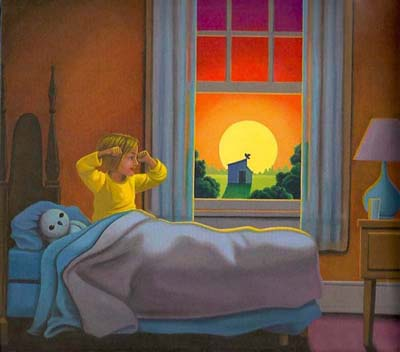
\includegraphics[width=0.26\columnwidth]{../figures/exintrans.jpeg} & 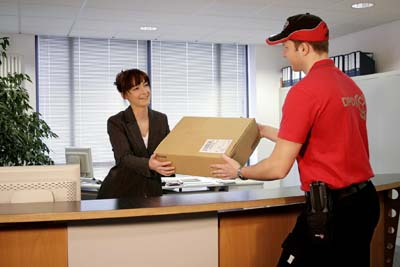
\includegraphics[width=0.3\columnwidth]{../figures/exditrans.jpg} \\
\smallskip \\
passive? & compound subj? \\
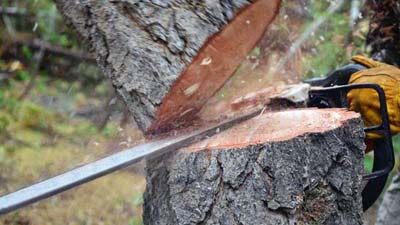
\includegraphics[width=0.3\columnwidth]{../figures/expassive.jpg} & 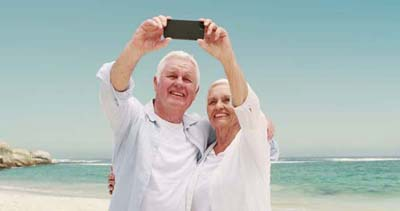
\includegraphics[width=0.3\columnwidth]{../figures/excompound.jpg} \\
\end{tabular}
\end{center}
\end{figure}
\end{frame}


\subsection{Timeline}
\begin{frame}
\frametitle{Future work}
\framesubtitle{Timeline}
\begin{center}
\footnotesize
\begin{tabular}{|l|l|l|}
  \hline
  \textbf{Task} & \textbf{Start} & \textbf{Finish} \\
  \hline
  \hline
  System (incl. SRL/WordNet, clustering) & ... & Dec 2016 \\
  \hline
  \textit{Write introduction} & Aug 2016 & Sep 2016 \\
  \hline
  \textit{Write SLA section (motivation, lit review)} & Aug 2016 & Oct 2016 \\
  \hline
  Prep PDT; IRB; collect data & Jun 2016 & Oct 2016 \\
  \hline
  \textit{Write NLP section (lit review)} & Sep 2016 & Nov 2016 \\
  \hline
  \textit{Write method section (incl. training data)} & Jul 2016 & Dec 2016 \\
  \hline
  Annotation & Sep 2016 & Nov 2016 \\
  \hline
  \textit{Write data collection \& description section} & Sep 2016 & Nov 2016 \\
  \hline
  System experiments with new data & Nov 2016 & Dec 2016 \\
  \hline
  \textit{Write experiments \& results section} & Dec 2016 & Jan 2017 \\
  \hline
  Implement feedback system & Jan 2017 & Feb 2017 \\
  \hline
  \textit{Write feedback section} & Jan 2017 & Feb 2017 \\
  \hline
  \textit{Write conclusion (finish 1st draft)} & Jan 2017 & Feb 2017 \\
  \hline
  Complete any follow-up experiments & Feb 2017 & Mar 2017 \\
  \hline
  \textit{Revise draft} & Mar 2017 & Apr 2017 \\
  \hline
  \textit{Final draft complete} / Defense & & May 2017 \\
  \hline
\end{tabular}
\end{center}
\end{frame}

%
%\begin{frame}
%\frametitle{GS difficulties \textbf{(Revise \& incorporate)}}
%\scriptsize{(Some of this should be cut, some used to motivate current approaches, and some retained for a ``future challenges'' type slide toward the end)}
%\medskip
%
%Recombination $\Rightarrow$ unwanted triples in the gold standard set?
%\begin{itemize}
%\item Gold (NS): \textit{wash(woman,shirt)}
%\item Gold (NS): \textit{do(woman,laundry)}
%\item Recombined: \textit{do(woman,shirt)}?
%\end{itemize}
%
%%\bigskip
%
%Matching semantics $\neq$ Matching nativeness?
%\begin{itemize}
%\item NNSs produce a wider range of forms to describe the prompts than
%  NSs, e.g.,
%  \begin{itemize}
%  \item NSs: overwhelmingly described \textit{raking} action
%  \item NNSs: often described \textit{cleaning} an area
%  \end{itemize}
%\item Related to issues of lexical gaps \citep{AgustinLlach2010} \&
%  attaining native-like pragmatic usage \citep{BardoviDornyei1998}
%\item What counts as a correct meaning is application-specific
%\end{itemize}
%
%
%\end{frame}

%\section{Outlook}
%\begin{frame}
%\frametitle{Summary \& Outlook [NOT UPDATED, 8/24]}
%
%Summary:
%\begin{itemize}
%\item Shifted from rule-based, semantic triple analysis to probabilistic, dependency-based analysis
%\item Scored responses with GS similarity rather than strict match/non-match; ranked responses
%\item Clustered data based on response and system features
%\end{itemize}
%
%\smallskip
%Outlook:
%\begin{itemize}
%\item Align response clusters with system clusters
%\item Cluster approaches \& parameters, align with item clusters (for auto selection of settings for new items)
%\item Methods for discriminating acceptable/unacceptable responses based on response rankings
%\item Incorporate WordNet \& SRL info
%\item Implement (minimal) feedback module
%\end{itemize}
%\end{frame}

%\section{Acknowledgements}
%\begin{frame}
%\frametitle{Acknowledgements}
%We would like to thank everyone who helped with this work:
%\medskip
%\begin{itemize}
%\item PDT help: David Stringer 
%\medskip
%\item Recruiting help: Kathleen Bardovi-Harlig, Marlin Howard, Jayson Deese 
%\medskip
%\item Feedback: Ross Israel, three anonymous reviewers, attendees of the IU Graduate Student Conference, CLingDing attendees
%\end{itemize}
%\end{frame}
%
\begin{beamercolorbox}{title}
\mbox{}\\[1ex]%\vspace{1ex}
\usebeamerfont{title}References
\end{beamercolorbox}
\medskip
\scriptsize
\bibliographystyle{../styles/myaclnat}
\bibliography{../levi-bib}

\begin{frame}[noframenumbering]
\frametitle{Response and GS comparison}
\vspace{-2em}
The $2 \times 2$ dimensions result in these approaches:
\smallskip
\begin{itemize}
\item \textbf{FA} (freq avg): Baseline. 
  \begin{itemize}
  \item Each NNS term is scored with the term's frequency in the
    GS. Response term scores are averaged. 
  \item Higher scores are closer to GS.
  \end{itemize}
\item \textbf{TA} (tf-idf avg): Run tf-idf on GS.
  \begin{itemize}
  \item Each NNS term is scored with the term's tf-idf score in GS.
    Response term scores are averaged.
  \item Higher scores are closer to GS.
  \end{itemize}
\item \textbf{FC} (freq compar.): Calculate term freq for NNS, GS; Treat as vectors, score response with cosine distance.
\smallskip
\item \textbf{TC} (tf-idf compar.): Run tf-idf on NNS, GS; Treat these as vectors, score response with cosine distance.
\end{itemize}
\end{frame}

\begin{frame}[noframenumbering]
\frametitle{Comparison results}
\framesubtitle{Evaluating settings}
\begin{table}%[htb!]
\begin{center}
\begin{tabular}{|r|l|c|}
 \hline
 Rank & MAP & Settings \\
 \hline
 \hline
1 & 0.5534 & TC\_B\_NNSLM\_lxh \\
\hline
2 & 0.5445 & TA\_B\_NNSLM\_lxh \\
\hline
3 & 0.5435 & TC\_W\_NNSLM\_lxh \\
\hline
4 & 0.5422 & TC\_B\_NNSLM\_xdh \\
\hline
5 & 0.5368 & TC\_B\_NNSLM\_ldh \\
 \hline
 \hline
56 & 0.4816 & TA\_B\_NNSO\_xdx \\
\hline
57 & 0.4796 & FA\_na\_NNSLM\_ldx \\
\hline
58 & 0.4769 & FC\_na\_NNSO\_lxh \\
\hline
59 & 0.4721 & TA\_W\_NNSO\_xdx \\
\hline
60 & 0.4530 & FA\_na\_NNSO\_lxh \\
\hline
\end{tabular}
%\begin{minipage}{.86\columnwidth}
\vspace{.7em}
\caption{Based on Mean Average Precision, the five best and five worst settings across all 10 PDT items.}
%\label{tab:all-dist-ranked-settings}
%\end{minipage}
\end{center}
\end{table}
\end{frame}

\begin{frame}
\frametitle{Comparison results}
\framesubtitle{Preliminary observations}
\begin{itemize}
	\item{Best approach: \textbf{TC}}
	\begin{itemize}
		\item{\textbf{TC} \textgreater \ \textbf{FC}, \textbf{TA} \textgreater \ \textbf{FA}:} 
		\begin{itemize}
			\item{tf-idf weighting \textgreater \ frequency weighting}
		\end{itemize}
		\item{\textbf{TC}\&\textbf{FC} \textgreater \ \textbf{TA}\&\textbf{FA}:}
		\begin{itemize}
			\item{cosine distance \textgreater \ weight averaging}
		\end{itemize}
	\end{itemize}
	\item{Term form: \textbf{xdh, ldh, lxh} \textgreater \ \textbf{xdx, ldx}}
	\begin{itemize}
        \item{Importance of heads (\textbf{h}): with short transitive
            responses, verbs are salient (subj/obj head)}
	\end{itemize}
	\item{Reference corpus: \textbf{Brown} \textgreater \ \textbf{WSJ}}
	\begin{itemize}
        \item{Content \& style of responses more like \textbf{Brown}}
%            than \textbf{WSJ}}
	\end{itemize}
	\item{NNS source: \textbf{NNSLM} \textgreater \ \textbf{NNSO}}
	\begin{itemize}
        \item{More errors in NNSLM forms, inflating MAP values:
            use non-normalized scores?}
	\end{itemize}
\end{itemize}

\end{frame}

\begin{frame}[noframenumbering]
\frametitle{Comparison results}
\framesubtitle{Evaluating settings}
Ranked approach \& parameter scores (averaged across all 10 PDT items)
\begin{center}
\footnotesize
%\begin{tabular}{|l|r||l|r||l|r||l|r|}
% \hline
% \multicolumn{2}{|c||}{Approach} & \multicolumn{2}{|c||}{term form} & \multicolumn{2}{|c||}{tf-idf reference} & \multicolumn{2}{|c|}{NNS source} \\
% \hline
% \hline
% FA & 160.38 & lemma & 165.80 & Brown & 173.24 & LM & 165.96 \\
% \hline
% FC & 163.84 & xdh & 165.83 & WSJ & 176.25 & Orig & 173.81 \\
% \hline
% TA & 174.74 & ldh & 166.17 & & & & \\
% \hline
% TC & 174.74 & lxh & 169.89 & & & & \\
% \hline
% & 	& ldx & 179.02 & & & & \\
% \hline
%\end{tabular}
\begin{table}
\begin{tabular}{|l|r||l|r||l|r||l|r|}
 \hline
 \multicolumn{2}{|c||}{Approach} & \multicolumn{2}{|c||}{Term Form} & \multicolumn{2}{|c||}{tf-idf reference} & \multicolumn{2}{|c|}{NNS Source} \\
 \hline
 \hline
 TC & 0.51577 & xdh & 0.51810 & Brown & 0.51534 & LM & 0.51937 \\
 \hline
 FC & 0.50780 & ldh & 0.51677 & WSJ & 0.50798 & Orig & 0.49699 \\
 \hline
 TA & 0.50755 & lxh & 0.51350 & & & & \\
 \hline
 FA & 0.49464 & xdx & 0.49901 & & & & \\
 \hline
 & 	& ldx & 0.49352 &  &  &  & \\
 \hline
\end{tabular}
\vspace{.7em}
\caption{Approaches and parameters ranked by mean average precision for all 10 PDT items.}
\label{tab:dist-ranked-parameters}
\end{table}
\end{center}
\end{frame}

\begin{frame}[noframenumbering]
\frametitle{Clustering}
\framesubtitle{Feature selection}
%\vspace{-1em}
Currently, experimenting with combinations of features for hierarchical clustering of PDT items. (And settings?)
\begin{itemize}
\item To help get a handle on learner variability for different items and correlation to best-performing models
\end{itemize}
\medskip
Response features:
\begin{itemize}
\item{For each response source (GS, NNSO, NNSLM):}
\begin{itemize}
\item{For each term form (lemma, ldh, xdh, lxh, ldx):}
\item{(We also use previous triples as ``terms'' here)}
\begin{itemize}
\item{type count}
\item{token count}
\item{type-to-token ratio}
%\item{suggestions?}
\end{itemize}
\end{itemize}
\end{itemize}

\medskip
System features:
\begin{itemize}
\item{Per item average error scores for settings using:}
\begin{itemize}
\item{Each approach (FA, TA, FC, TC)}
\item{Each tf-idf reference (Brown, WSJ)}
\item{Each NNS response source (NNSO, NNSLM)}
\item{Each term form (lemma, ldh, xdh, lxh, ldx)}
%\item{suggestions?}
\end{itemize}
\end{itemize}

\end{frame}

\begin{frame}[noframenumbering]
\frametitle{Clustering items by responses}
\footnotesize
\begin{figure}[width=0.9\columnwidth]
\begin{center}
\begin{tabular}{|c|}
\hline
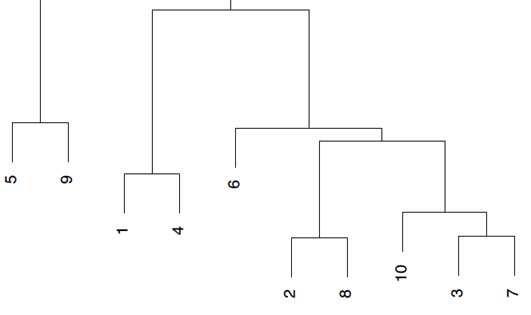
\includegraphics[width=0.65\columnwidth]{../figures/allcounts.jpg} \\
\hline
All NNSO, NNSLM, GS type \& token counts\\
\hline
\hline
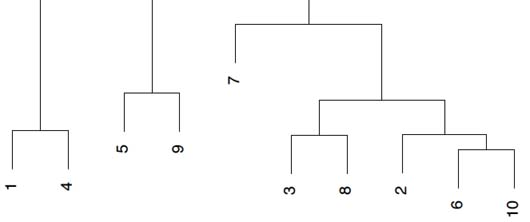
\includegraphics[width=0.65\columnwidth]{../figures/nnsottr.jpg} \\
\hline
NNSO type-to-token ratio \\
\hline
\end{tabular}
\end{center}
\end{figure}
\end{frame}

\begin{frame}[noframenumbering]
\frametitle{Clustering items by system performance}
\footnotesize
\begin{figure}[width=0.9\columnwidth]
\begin{center}
\begin{tabular}{|c|}
\hline
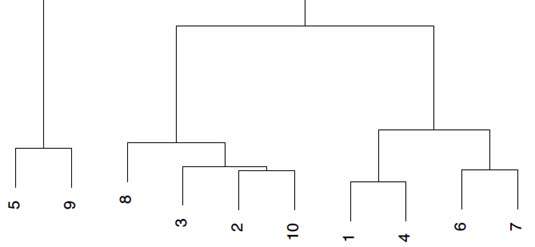
\includegraphics[width=0.65\columnwidth]{../figures/parameters.jpg} \\
\hline
All average scores for approaches \& parameters\\
\hline
\hline
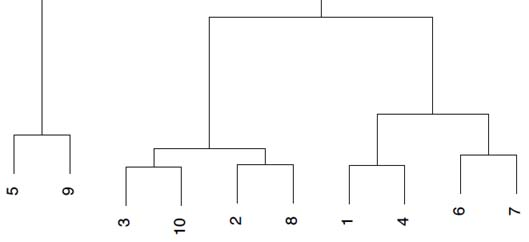
\includegraphics[width=0.65\columnwidth]{../figures/approach.jpg} \\
\hline
All average scores for approaches \\
\hline
\end{tabular}
\end{center}
\end{figure}
\end{frame}

\begin{frame}[noframenumbering]
\frametitle{Clustering}
\framesubtitle{Observations}
%\vspace{-1em}
Some patterns among clusters: 
%Many combinations of features don't follow these patterns, however. 5 \& 9, 1 \& 4, and to a lesser extent, 2 \& 8 form pairs.
\begin{center}
\footnotesize
\begin{tabular}{|r|l||l|}
\hline
 & Sentence & Observations \\
\hline
\hline
5 & A man is raking leaves. & TA \& TC are high\\
\cline{1-2}
9 & Two boys are rowing a boat. & lemmas are high\\
\hline
\hline
1 & A boy is playing soccer. & FA \& FC are high\\
\cline{1-2}
4 & The man is reading the newspaper. & lemmas are low\\
\hline
\hline
2 & A woman is washing clothes. & \multirow{2}{*}{lemmas are high} \\
\cline{1-2}
8 & A person is cutting an apple. & \\
\hline
\end{tabular}
\end{center}
\begin{itemize}
\item NNSO vs NNSLM isn't salient? e.g., NNSO is best for 1, NNSLM for 4; same for 9, 5.
\item 5 \& 9 involved the most challenging verbs (\textit{raking}, \textit{rowing}); tf-idf approaches work best here, but why?
\begin{itemize}
\item cf. 1 \& 4, where frequency measures beat tf-idf
\end{itemize}
\end{itemize}
\end{frame}


\end{document}